\chapter{Introdução}
% \section{Introdução}
CubeSats são uma classe de artefatos espaciais elaborada com o intuito de reduzir custos e tempo de desenvolvimento,
além de providenciar maior acessibilidade ao espaço \cite{cubesat-spec}. Inicialmente projetados para utilização
educacional em universidades \cite{burt2011}, são amplamente usados para exploração espacial em órbita terrestre
baixa, com altitudes entre 160km e 2000km \cite{alanazi2019}.

CubeSats possuem uma unidade básica (U) de dimensão 10cm x 10cm x 10cm e de até 1kg de massa, mas podem ser configurados
em até 24 Unidades (ou 24U) \cite{cubesat}. O FloripaSat-2 \cite{floripasat2}, projeto do Laboratório de Pesquisa em
Tecnologias Espaciais da UFSC no qual este trabalho se baseia, é um CubeSat 2U que se encontra no presente momento,
em estágio de desenvolvimento ativo. A figura \ref{fig:floripasat2-diagram} apresenta uma renderização da configuração
do FloripaSat-2.

\begin{figure}[H]
\caption{\label{fig:floripasat2-diagram}Renderização do FloripaSat-2.}
\begin{center}
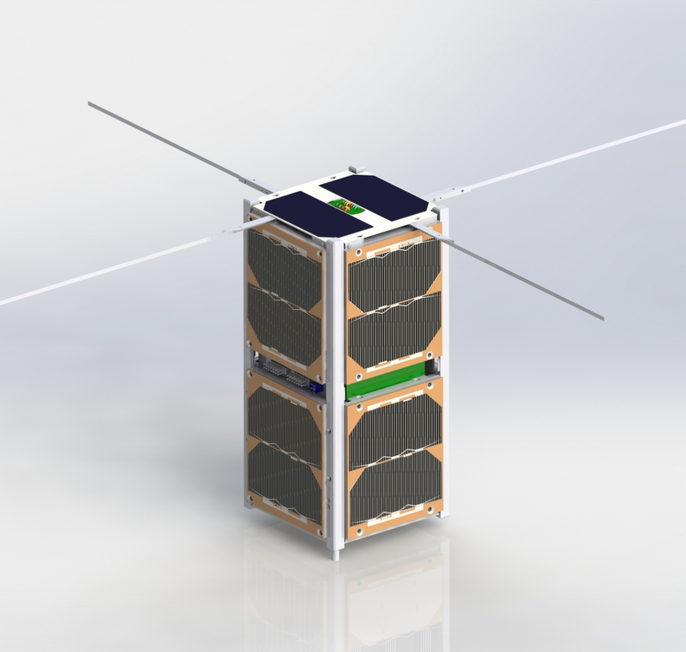
\includegraphics[scale=0.5]{images/floripasat-2-diagram.jpg}
\end{center}
\legend{Fonte: \cite{floripasat2}}
\end{figure}
\newpage

\textcolor{red}{
    Uma das etapas do desenvolvimento do FloripaSat-2 é a \emph{FlatSat} \cite{floripasat2},
    que se trata de uma plataforma de testes onde os módulos do satélite podem ser executados
    em conjunto para verificar e avaliar o funcionamento de ambos hardware e firmware dos módulos
    individuais, e ainda a interação entre eles, simulando o funcionamento do satélite em órbita.
}

O processo de verificação de design é uma etapa crucial em projetos de engenharia.
Em tradução livre dos autores, Monteiro et al, dizem que:

\begin{citacao}
\hspace{1,2cm}Em projetos espaciais, a amplitude e cuidado minucioso dos processos de teste são ainda mais
importantes, em vista do nível de confiabilidade  a ser imposto no produto final, que é comumente um artefato
espacial que precisa resistir à uma gama de ameaças e funcionar em um ambientes inóspitos. \cite{aiv-cubesat}
\end{citacao}

Ainda segundo os autores, o processo de \emph{AIV} (sigla em inglês para Montagem, Integração, e Verificação)
tende a ser mais leve em CubeSats, devido à menor escala dos projetos.


No entanto, o risco de um projeto de nanossatélite não é desprezível. Em um estudo realizado sobre os lançamentos
de CubeSats entre 2003 e 2015, os autores \cite{panga2016} constataram que cerca de 15\% das missões CubeSat nesse
período não conseguiram manter comunicações com as estações de controle, resultando em falha da missão após o lançamento.

Por esses motivos, percebe-se então a relevância de um plano de testes bem estuturado para o ciclo de desenvolvimento
do FloripaSat-2, pois é necessário elevar o nível de confiabilidade e a garantia de bom funcionamento do sistema, a fim
de diminuir a probabilidade de que problemas no satélite resultem em falha da missão.

Durante a participação e contribuição para o projeto, especialmente nos preparativos para \textcolor{red}{a elaboração
dos testes} e considerando os pontos descritos, o crescente interesse se expandiu e a possibilidade de torná-lo um
Trabalho de Conclusão de Curso surgiu.
O trabalho propõe, então, dois pontos principais:

\begin{itemize}
    \item A implementação de um sistema de workflows hospedados na plataforma GitHub Actions \cite {gh-actions} nos
          repositórios oficiais do projeto, que possibilite a execução automática de arquivos de teste e do firmware
          dos módulos do FloripaSat-2 durante a \emph{FlatSat};
    \item A análise qualitativa e quantitativa dos dados coletados e dos arquivos de \emph{log} gerados durante a
          execução dos testes.
\end{itemize}

Os resultados esperados deste trabalho são a criação de um modelo para automação a ser usado em futuros projetos de
desenvolvimento de sistemas embarcados para CubeSats, e um relatório com as conclusões e análises obtidas por meio do
estudo dos dados e \emph{logs} coletados.

\section{Objetivos}

\subsection{Objetivo Geral}

O objetivo principal do trabalho é implementar um sistema de fluxos de testes automatizados, hospedados na plataforma
GitHub em conjunto com os repositórios dos sistemas e módulos do FloripaSat-2. Eles então, serão aplicados durante o
projeto de desenvolvimento do satélite e através dos resultados coletados durante a execução dos testes, e será
apresentada uma análise conclusiva sobre a etapa de \emph{FlatSat}.
\subsection{Objetivos Específicos}

\begin{enumerate}
    \item Implementar \textit{workflows} capazes de automatizar a execução de softwares e testes;
    \item Implementar sistemas de geração e armazenamento de dados de \textit{log} das execuções dos \textit{workflows};
    \item Analisar e interpretar os registros coletados para a obtenção de resultados conclusivos sobre a etapa de execução;
    \item Disponibilizar códigos-fonte, dados de registro e resultados obtidos.
\end{enumerate}
\section{Organização do trabalho}

Este trabalho está organizado do seguinte modo:

\begin{itemize}
    \item O capítulo 2 apresenta a definição da metodologia utilizada e a formalização da fundamentação teórica utilizada
          na elaboração do trabalho;
    \item O capítulo 3 apresenta uma breve revisão de alguns trabalhos relacionados que abordam o desenvolvimento e testes
          de CubeSats;
    \item O capítulo 4 apresenta e descreve o sistema proposto;
    \item O capítulo 5 contém as conclusões, considerações finais e os trabalhos futuros.
\end{itemize}
